\documentclass{beamer}
\usepackage{cancel, algpseudocode, hyperref, tikz, venndiagram, centernot}

\title{CS 70 Discussion 8B}
\date{October 25, 2024}

\begin{document}

\frame{\titlepage}

\begin{frame}
    \frametitle{Conditional Probability}
    {\bf Problem}: How do we represent the probability of an event $B$, {\it given} that event $A$ happens?\\
    {\bf Notation}: $\mathbb{P}[B|A]=\mathbb{P}[B\text{ happens given }A\text{ happened}]$. We can say:
    \begin{gather*}
        \mathbb{P}[B|A]=\frac{\mathbb{P}[A\cap B]}{\mathbb{P}[A]}\\
        \mathbb{P}[A\cap B]=\mathbb{P}[B|A]\mathbb{P}[A]=\mathbb{P}[A|B]\mathbb{P}[B]
    \end{gather*}
    \begin{center}
        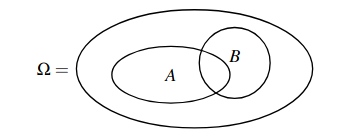
\includegraphics[scale=0.5]{Images/conditional-probability.png}
    \end{center}
\end{frame}

\begin{frame}
    \frametitle{Bayes' Rule}
    I want to use $\mathbb{P}[A|B]$ to calculate $\mathbb{P}[B|A]$:
    \begin{gather*}
        \mathbb{P}[B|A]=\frac{\mathbb{P}[A|B]\mathbb{P}[B]}{\mathbb{P}[A]}
    \end{gather*}
    {\bf Application}: I want to calculate the accuracy of a COVID test. I know $\mathbb{P}[\text{test is positive}|\text{a person has COVID}]$ from an experiment. But, the efficacy of the test is determined by $\mathbb{P}[\text{a person has COVID}|\text{test is positive}]$ (we want to predict whether someone has COVID from the test, not predict the output of the test after already knowing someone has COVID!).
\end{frame}

\begin{frame}
    \frametitle{Total Probability Rule}
    {\bf Problem}: I want to calculate the probability of the event $B$, but I can only calculate $\mathbb{P}[B\cap A_i]$ for a list of events $A_1,A_2,\dots,A_n$ where for any $i\neq j$, $A_i\cap A_j=\emptyset$ and $\bigcup_{i=1}^n A_i=\Omega$.\\
    {\bf Formula}:
    \begin{gather*}
        \mathbb{P}[B]=\sum_{i=1}^n\mathbb{P}[B\cap A_i]=\sum_{i=1}^n\mathbb{P}[B|A_i]\mathbb{P}[A_i]
    \end{gather*}
    \begin{center}
        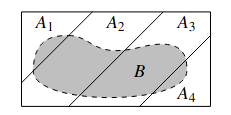
\includegraphics[scale=0.6]{Images/total-probability.png}
    \end{center}
\end{frame}

\begin{frame}
    \frametitle{Independence}
    {\bf Motivation}: We need a formal definition of what it means for two events to be {\it independent}, meaning the occurrence of one event doesn't effect the probability of the other event occurring.\\
    {\bf Definition}: Events $A_1,A_2,...,A_n$ are {\bf mutually independent} iff:
    \begin{gather*}
        \mathbb{P}\left[\bigcap_{i=1}^n A_i\right]=\prod_{i=1}^n\mathbb{P}[A_i]
    \end{gather*}
    $A_1,A_2,\dots,A_n$ are {\bf pairwise independent} iff:
    \begin{gather*}
        (\forall i\neq j)(\mathbb{P}[A_i\cap A_j]=\mathbb{P}[A_i]\mathbb{P}[A_j])
    \end{gather*}
    Mutual Independence$\implies$Pairwise Independence, but Pairwise Independence$\centernot\implies$Mutual Independence
\end{frame}

\end{document}
